\chapter{Špecifikácia konkrétnych API tokenov}

\label{kap:typy} % id kapitoly pre prikaz ref

V tejto kapitole predstavíme v praxi využívané API tokeny, ktorými sa zaoberá naša práca. Uvedieme ich formát a základné postupy pre ich vytvorenie, či validáciu. Ich využitie, výhody či nevýhody rozoberieme v kapitole \ref{kap:teoreticke}.


\section{JSON Web Token}

Prvý token, ktorým sa budeme zaoberať je JSON web token (JWT) \cite{jwt_rfc}. JWT vznikol ako súčasť JOSE (JSON object signing and encryption) štandardov \cite{jose_rfc}, čo je dokument vypracovaný pracovnou skupinou IETF (Internet Engineering Task Force) na základe aplikácií bezpečnostných mechanizmov v rámci vývoja softvéru.

Definujú štandard pre bezpečný prenos JSON objektov medzi službami, ktoré sú schopné ich overiť a dešifrovať. Zavádzajú tri základné formáty JSON objektov a to JWS (JSON Web Signature), JWE (JSON Web Encryption) a JWK (JSON Web Key), ktorým sa detailnejšie venujú ďalšie štandardy \cite{jws_rfc, jwe_rfc, jwk_rfc}. Prvé dva sú formáty zabezpečujúce bezpečnostné vlastnosti JSON objektov. Oba zabezpečujú autentickosť a integritu pomocou digitálnych podpisov alebo hešovaného autentifikačného kódu. JWE navyše zabezpečuje aj dôvernosť a to šifrovaním obsahu JSON objektu. Posledný formát JWK je formát pre reprezentáciu kľúčov, ktoré sú použité v kryptografických algoritmoch využitých v JWS a JWE. Kryptografické algoritmy a ich identifikátory sú definované JSON Web Algorithms (JWA) štandardom \cite{jwa_rfc}.


\subsection{Štruktúra JWT}

Samotný JWT je v podstate iba serializovaný JSON objekt chránený JWS alebo JWE. Podľa štandardu JWT obsahuje tri samostatné časti oddelené bodkami - hlavičku, telo a podpis. Hlavička a telo sú serializované JSON objekty obsahujúce oprávnenia (angl. claim) vo forme dvojíc kľúč, hodnota. Niektoré oprávnenia (konkrétne ich kľúče) sú definované v štandarde a teda by sa nemali používať pre žiadne iné hodnoty. 

A to konkrétne v hlavičke sú najdôležitejšie \textit{typ} a \textit{alg}. Prvý určuje typ tokenu a druhý algoritmus, ktorý bol použitý na vytvorenie podpisu alebo v rámci šifrovania obsahu tokenu. Rôzne možnosti pre algoritmy sú definované v JWA štandardoch.

Telo tvorí logický obsah tokenu, napríklad môže obsahovať oprávnenia týkajúce sa konkrétnej autentifikácie a používateľa, pre ktorého bol token vydaný. Dôležité štandardom popísané kľúče sú napríklad \textit{iss}, \textit{sub}, \textit{exp}, \textit{nbf}, \textit{iat}. Popisujú postupne vydavateľa tokenu, identifikátor používateľa, čas vypršania platnosti tokenu, čas, kedy sa token začne považovať za platný a čas vydania tokenu.

Do tela aj hlavičky sa môžu vkladať ľubovoľné iné oprávnenia, napríklad \textit{admin}, \textit{role}, \textit{permissions}, určujúce oprávnenia používateľa.

\subsection{Generovanie a validácia JWT}

Hlavička a telo sa serializujú pomocou base64url kódovania \cite{base64_rfc}. V prípade JWE sa telo ešte pred serializáciou šifruje. Následne sa obe časti podpíšu algoritmom definovaným v hlavičke a podpis sa zreťazí s hlavičkou a telom. Výsledný reťazec sa používa ako token.

Na overenie platnosti tokenu treba overiť podpis. Podpis je vytvorený pomocou algoritmu definovanom v hlavičke. Teda pri validácii tokenu sa ako prvé dekóduje hlavička tokenu a z nej sa prečíta hodnota v kľúči \textit{alg}.

Na základe hodnoty v kľúči \textit{alg} sa určí algoritmus, ktorý bol použitý na podpis tokenu. Následne sa podpis zvaliduje. 

Ak bol token vytvorený pomocou JWE, na prečítanie tela je potrebné ho najprv dešifrovať pomocou algoritmu, ktorý je zapísaný ako oprávnenie s kľúčom \textit{enc} v hlavičke tokenu. V prípade využitia JWS je telo po dekódovaní priamo čitateľné. Následne môžeme overiť informácie o časovej platnosti tokenu, či právach používateľa a pod.

Príklad vytvorenia nešifrovaného JWT tokenu s podpisovou funckiou HMAC-SHA256 a telom obsahujúcim oprávnenie \textit{iss} a \textit{iat} je zorbazený na obrázku \ref{fig:jwt_token}.

\begin{figure}
    %vlozenie samotneho obrazku vycentrovaneho a vhodnej velkosti
    %obrazok je v subore images/session.png
    \centerline{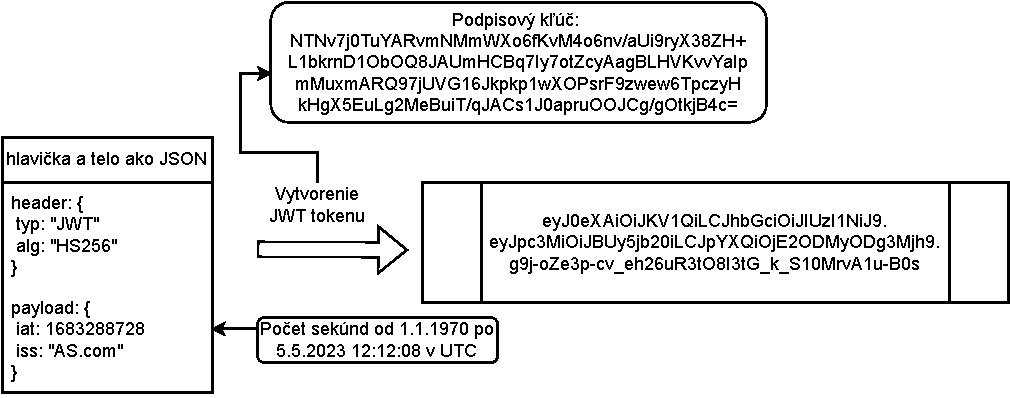
\includegraphics[width=0.8\textwidth]{images/jwt_token}}
    %popis obrazku
    \caption[JWT token]{Príklad jednoduchého JWT tokenu.}
    %id obrazku, pomocou ktoreho sa budeme na obrazok odvolavat
    \label{fig:jwt_token}
\end{figure}


\section{Platform Agnostic Security Token}

Platform Agnostic Security Token (PASETO) je relatívne nový štandard tokenu navrhnutý v roku 2018 a je stále v štádiu RFC draftu \cite{paseto_rfc}. Je inšpirovaný rodinou štandardov JOSE (JWT, JWS, JWE, JWK). Jednoducho povedané snaží sa zjednodušiť implementáciu a použitie kryptografických funkcií.

Rovnako ako JWT, PASETO serializuje JSON objekty a zaručuje rôzne bezpečnostné kvality pri ich prenose cez internet. Pôvodne bol PASETO navrhnutý s dvoma verziami \textit{v1} a \textit{v2} líšiacimi sa v použitých kryptografických algoritmoch. Dnes už existujú štyri verzie \textit{v1}, \textit{v2}, \textit{v3} a \textit{v4} popísané štandardom \cite{paseto_git}. Každá verzia tokenu zaručuje autentickosť a integritu obsahu tokenu a to pomocou asymetrického šifrovania v zmysle digitálneho podpisu alebo pomocou hešovaného autentifikačného kódu.

\subsection{Verzie PASETO}

Ako sme spomenuli PASETO má štyri verzie. Každá verzia sa delí na dve ďalšie podľa jej využitia na lokálnu a verejnú. Lokálne tokeny majú zašifrované telo a tým zabezpečujú dôvernosť dát uložených v tele tokenu. Na rozdiel od toho sú verejné tokeny nešifrované a dáta v ich tele sú čitateľné pre kohokoľvek s prístupom k danému tokenu.

Každá verzia PASETO používa iný algoritmus na podpisovanie a prípadne šifrovanie tokenu v prípade lokálnych tokenov. Jednotlivé algoritmy pre konkrétne verzie a ich použitie sú popísané v špecifikácii \cite{paseto_git}.

Novšie verzie \textit{v3} a \textit{v4} prinášajú modernejšie kryptografické algoritmy a pridávajú niektoré funkcionality. Napríklad verzia \textit{v3} prináša nepopierateľnosť autorstva ako novú bezpečnostnú kvalitu. Dosahuje to dokonca bez predĺženia podpisu a to pomocou pridania verejného kľúča do tokenu pred vypočítaním podpisu \cite{ueo}. Tiež zavádza podporu pre implicitné informácie, teda také informácie, ktoré nie sú uložené priamo v tokene, ale používajú sa pri výpočte podpisu. Teda sú to informácie potrebné pre validáciu tokenu, ale z nejakého dôvodu nie je vhodné ich vkladať priamo do tokenu. Napríklad môže ísť o citlivé interné dáta. Podrobná motivácia za zavedením nových verzií je popísaná v špecifikácii \cite{paseto_git}.

\subsection{Štruktúra PASETO}

PASETO sa skladá z troch alebo štyroch častí zreťazených bodkou. Časti postupne reprezentujú verziu, využitie, telo a pätu. Prvé tri časti sú povinné a päta je nepovinná, ale dovoľuje nám zapísať akékoľvek ďalšie informácie do tokenu.

\begin{itemize}
    \item Verzia -- reprezentuje verziu PASETO. Môže byť \textit{v1}, \textit{v2}, \textit{v3} alebo \textit{v4}.
    \item Využitie -- určuje využitie tokenu ako lokálne alebo verejné. Možné hodnoty sú \textit{local} alebo \textit{public}.
    \item Telo -- reprezentuje samotné dáta uložené v tokene. Podobne ako pri JWT ide o oprávnenia vo forme dvojíc kľúč hodnota a rovnako sú niektoré dôležité kľúče definované špecifikáciou. \cite{paseto_git}
    \item Päta -- môže obsahovať ľubovoľné ďalšie informácie.
\end{itemize}

Telo a päta sú vo forme JSON objektu, ktorý je serializovaný pomocou base64url \cite{base64_rfc}.


\subsection{Generovanie a validácia PASETO}

Pri vytváraní tokenu sa musíme najprv rozhodnúť pre verziu a využitie podľa toho aké bezpečnostné požiadavky máme na token. Následne vytvoríme telo tokenu obsahujúce informácie, ktoré chceme pomocou tokenu prenášať, napríklad informácie o vzniku tokenu, jeho platnosti, jeho autorovi, či určenom subjekte. Ďalej môžeme pridať ďalšie informácie do päty tokenu ako napríklad identifikátor kľúča kryptografickej funkcie. 

Ak sme zvolili lokálne využitie, tak telo tokenu zašifrujeme. Následne vypočítame podpis z tela a päty tokenu. Šifrovanie aj podpisovanie sa deje pomocou kryptografickej funkcie vybratej podľa verzie a využitia. Nakoniec všetky časti spojíme do jedného reťazca a oddelíme bodkami.

Validácia tokenu je inverzný proces ku generovaniu. Najprv rozdelíme reťazec na časti a zistíme verziu a využitie tokenu a podľa toho vyberieme použitú kryptografickú funkciu. Následne zistíme, či je podpis tokenu platný pomocou adekvátnej kryptografickej funkcie a kľúča. Ak mal token lokálne využitie dešifrujeme jeho telo a skontrolujeme časovú platnosť tokenu, ak to využívaná schéma podporuje a telo obsahuje informácie o platnosti tokenu.

Príklad vytvorenia PASETO tokenu verzie \textit{v2} s verejným využitím a telom obsahujúcim oprávnenie \textit{iss} a \textit{iat} je zobrazený na obrázku \ref{fig:paseto_token}.

\begin{figure}
    %vlozenie samotneho obrazku vycentrovaneho a vhodnej velkosti
    %obrazok je v subore images/session.png
    \centerline{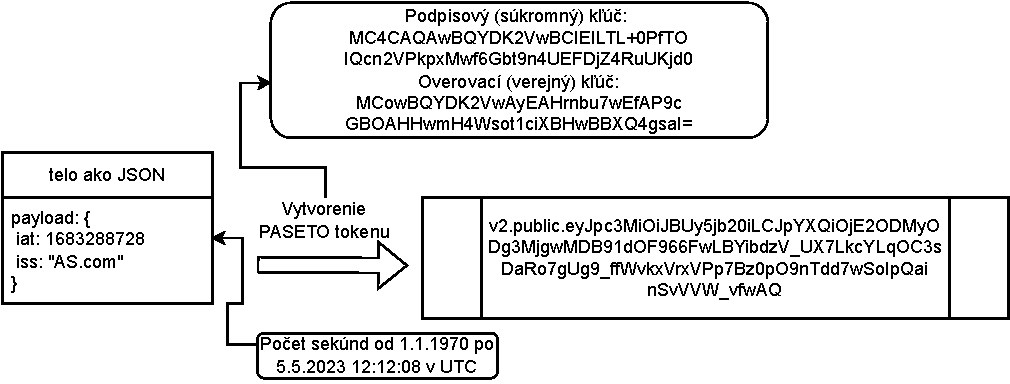
\includegraphics[width=0.8\textwidth]{images/paseto_token}}
    %popis obrazku
    \caption[PASETO token]{Príklad jednoduchého PASETO tokenu.}
    %id obrazku, pomocou ktoreho sa budeme na obrazok odvolavat
    \label{fig:paseto_token}
\end{figure}

\section{Fernet}

Pôvodne Fernet vznikol ako nástroj na zasielanie bezpečných správ v platforme cloudových služieb Heroku \cite{fernet_legacy}. V súčasnosti už podľa špecifikácie \cite{fernet_spec} vzniklo veľa implementácií Fernetu v rôznych programovacích jazykoch \cite{fernet_cpp, fernet_haskell}, v rámci Heroku bol implementovaný v Ruby. Fernet bol dokonca vybratý PYCA (Python Cryptographic Authority) \cite{pyca_crypto} ako štandard pre implementáciu symetrického šifrovania v Pythone.

Fernet je štruktúrovaný token, lebo v sebe nesie rôzne informácie, no nijak nešpecifikuje formát týchto informácií. Väčšina implementácií s nimi pracuje ako s obyčajným reťazcom znakov. 

Token je navrhnutý s možnosťou pridania viacerých verzií, no v súčasnosti existuje len jediná verzia. V tejto verzií je obsah tokenu zašifrovaný pomocou AES-128-CBC \cite{aes_cbc} a celý token je podpísaný pomocou HMAC-SHA256 \cite{hmac}. Z toho vyplýva, že Fernet zaručuje autentickosť, integritu a dôvernosť.

\subsection{Štruktúra Fernet}

Fernet sa skladá z piatich zreťazených častí. Každá časť reprezentuje jednu informáciu o tokene. Jednotlivé časti sú nasledovné:

\begin{itemize}
    \item Verzia -- reprezentuje verziu Fernet tokenu, aktuálne existuje len jedna verzia a je reprezentovaná číslom 0x80. Zaberá vždy 8 bitov.
    \item Časová pečiatka -- reprezentuje čas vytvorenia tokenu. Čas je zachytení ako počet sekúnd od 1.1.1970 v UTC časovej zóne. Zaberá vždy 64 bitov.
    \item Inicializačný vektor (IV) -- reprezentuje náhodný reťazec znakov, ktorý je použitý pri šifrovaní a dešifrovaní tokenu. IV musí byť unikátny a najmä nepredvídateľný pre každý token, preto sa generuje náhodnou funkciou. Zaberá vždy 128 bitov.
    \item Zašifrované telo -- reprezentuje zašifrované dáta uložené v tokene. Môže mať premenlivú dĺžku, no vždy násobok 128 bitov.
    \item Podpis -- reprezentuje výstup HMAC-SHA256 funkcie a zaberá vždy 256 bitov.
\end{itemize}

Ako vidíme, všetky časti tokenu okrem tela majú pevne danú dĺžku. Vďaka tejto vlastnosti nemusia byť zreťazené časti oddelené žiadnym špeciálnym symbolom, napríklad bodkou, lebo vieme jednoznačne oddeliť verziu, časovú pečiatku, IV aj podpis a tým pádom aj zašifrované telo.

Pre jednoduché prenášanie je celý token zakódovaný pomocou base64url \cite{base64_rfc}.

Príklad Fernet tokenu pred base64url zakódovaním s telom obsahujúcim reťazec \textit{issuer:AS.com} je schematicky vyjadrený na obrázku \ref{fig:fernet_token}.

\begin{figure}
    %vlozenie samotneho obrazku vycentrovaneho a vhodnej velkosti
    %obrazok je v subore images/session.png
    \centerline{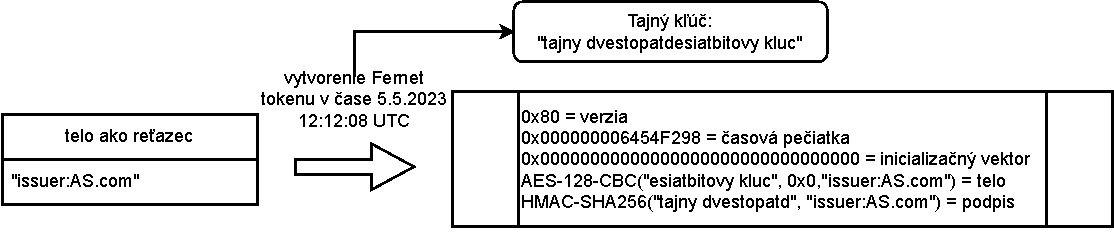
\includegraphics[width=0.8\textwidth]{images/fernet_token}}
    %popis obrazku
    \caption[Fernet token]{Príklad jednoduchého Fernet tokenu.}
    %id obrazku, pomocou ktoreho sa budeme na obrazok odvolavat
    \label{fig:fernet_token}
\end{figure}

\subsection{Generovanie a validácia Fernet}

Pri generovaní Fernet tokenu sa využívajú dva kryptografické algoritmy, ktoré vyžadujú kľúč. Fernet definuje 256 bitový kľúč, ktorý je rozdelený na dve 128 bitové časti. Prvá časť reprezentuje podpisový kľúč a druhá šifrovací kľúč.

Existuje iba jedna verzia tokenu s pevne daným algoritmom. Pre vygenerovanie tokenu, potrebujeme zaznamenať aktuálny čas do časovej pečiatky a vygenerovať náhodný reťazec, ktorý bude slúžiť ako IV. Následne zašifrujeme telo tokenu pomocou šifrovacieho kľúča a IV. Ďalej vypočítame podpis z predchádzajúcich častí tokenu pomocou podpisového kľúča. Nakoniec všetky časti spojíme do jedného reťazca a zakódujeme pomocou base64url \cite{base64_rfc}.

Validácia tokenu spočíva v dekódovaní tokenu, rozdelení na časti a overení podpisu. Potom dešifrujeme telo tokenu pomocou šifrovacieho kľúča a IV. Následne prípadne overíme časovú platnosť tokenu, ak telo obsahuje potrebné informácie pre overenie časovej platnosti ako vznik a doba platnosti tokenu.

\section{Branca}

Motiváciou k vzniku Branca tokenu \cite{branca_spec} bolo modernizovanie použitých kryptografických konštrukcií Fernet tokenu. Branca má podobnú štruktúru aj generovanie a validáciu ako Fernet. Branca sa líši najmä v tom, že využíva šifrovaciu a podpisovú funkciu XChaCha20-Poly1305 AEAD \cite{chacha_poly}.

\subsection{Štruktúra Branca}

Branca sa podobne ako Fernet skladá z piatich zreťazených častí. Tieto časti sa však jemne líšia od častí Fernet tokenu a zakódované sú \textit{base62} kódovaním \cite{base62}.

\begin{itemize}
    \item Verzia -- reprezentuje verziu Branca tokenu, aktuálne existuje len jedna verzia a je reprezentovaná číslom 0xBA. Zaberá vždy 8 bitov.
    \item Časová pečiatka -- reprezentuje čas vytvorenia tokenu. Čas je zachytení ako počet sekúnd od 1.1.1970 v UTC časovej zóne. Zaberá vždy 32 bitov a je zapísaná ako číslo bez znamienka.
    \item Príležitostné slovo (angl. nonce) -- reprezentuje náhodný reťazec znakov, ktorý využíva šifrovacia funkcia. Ide v podstate o IV, ale využíva sa naozaj len raz, zatiaľ čo IV sa v blokovej šifre využije viac krát. Zaberá vždy 192 bitov.
    \item Zašifrované telo -- reprezentuje zašifrované dáta uložené v tokene. Môže mať ľubovoľnú dĺžku.
    \item Podpis -- v podobe hešovaného autentifikačného kódu - reprezentuje výstup funkcie Poly1305 a zaberá vždy 128 bitov.
\end{itemize}

Príklad Branca tokenu pred base64url zakódovaním s telom obsahujúcim reťazec \textit{issuer:AS.com} je schematicky vyjadrený na obrázku \ref{fig:branca_token}.

\begin{figure}
    %vlozenie samotneho obrazku vycentrovaneho a vhodnej velkosti
    %obrazok je v subore images/session.png
    \centerline{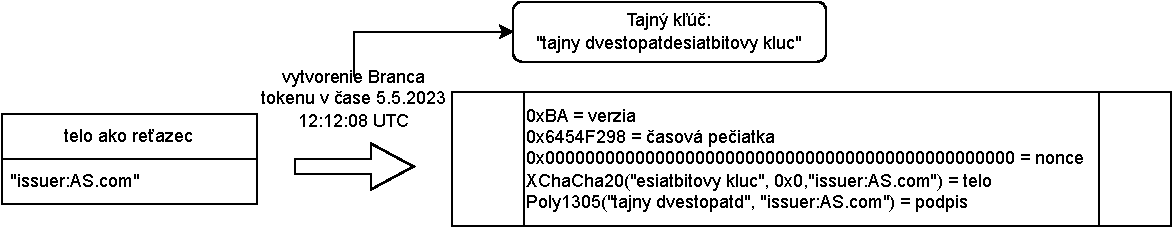
\includegraphics[width=0.8\textwidth]{images/branca_token}}
    %popis obrazku
    \caption[Branca token]{Príklad jednoduchého Branca tokenu.}
    %id obrazku, pomocou ktoreho sa budeme na obrazok odvolavat
    \label{fig:branca_token}
\end{figure}

\subsection{Generovanie a validácia Branca}

Vygenerujeme 192 bitový reťazec znakov, ktorý bude slúžiť ako príležitostné slovo a zachytíme aktuálny čas do časovej pečiatky. Vyrobíme hlavičku zreťazením verzie, časovej pečiatky a príležitostné slovo. Následne zašifrujeme telo tokenu pomocou šifrovacej funkcie, do ktorej vložíme tajný kľúč, príležitostné slovo a ako dodatočnú informáciu použijeme hlavičku. Funkcia vráti zašifrované telo a hešovaný autentifikačný kód vypočítaný aj z hlavičky. Nakoniec všetky časti spojíme do jedného reťazca a zakódujeme pomocou \textit{base62} kódovania \cite{base62}.

Pri validácií tokenu ho ako prvé dekódujeme. Následne overíme, že prvý bajt je 0xBA a token rozdelíme na jednotlivé časti. Dešifrujeme telo a overíme podpis pomocou funkcie XChaCha20-Poly1305 AEAD. Následne môžeme overiť napríklad časovú platnosť tokenu pomocou dodatočných informácií v tele tokenu a časovej pečiatky.

\section{Macaroons}

Macaroons sú tokeny s kontextovými pravidlami. Vznikli v rámci výskumného projektu Belay v spoločnosti Google \cite{belay}. Google predstavil Macaroons v práci z roku 2014 \cite{macaroons_paper}. Macaroons sú autorizačné poverenia (angl. credentials) pre cloudové služby s podporou decentralizovanej delegácie medzi službami v rámci cloudu. Ľubovoľná entita vlastniaca token autorizujúci určitý prístup môže tento token \textit{zoslabiť} alebo aj \textit{kontextovo obmedziť} a posunúť ďalšej entite. Zoslabenie aj kontextové obmedzenie sa realizuje pomocou pravidiel. Entitu generujúcu nový Macaroons token budeme označovať ako \textit{cieľová služba}.

Pravidlá sa delia podľa strany, ktorá potvrdí alebo zabezpečí ich naplnenie na pravidlá prvej a tretej strany. Pravidlá prvej strany sú jednoduché predikáty. Na autorizáciu požiadavky sprevádzanej Macaroons tokenom sa musia všetky tieto predikáty vyhodnotiť pravdivo v rámci kontextu danej požiadavky. Kontextom požiadavky môže byť napríklad aktuálny čas alebo IP adresa odosielateľa. Pravidlom prvej strany môže byť napríklad obmedzenie typu požiadaviek iba na čítacie. Pravidlá tretích strán vyžadujú dôkaz o nejakej skutočnosti od tretej strany. Pri dôkaze od tretích strán sa využíva princíp dôkazu držiteľa kľúča, kde tretia strana dokáže, že pozná nejaký tajný kľúč napríklad tak, že podpíše zadaný reťazec znakov. Pravidlom tretej strany môže byť požiadavka na doloženie dôkazu od nejakej autentifikačnej služby (napríklad autentifikačnej služby Google), že používateľ je autentifikovaný. Tento dôkaz musí získať používateľ pred odoslaním požiadavky na rozhranie a pri jej odoslaní ho priloží k požiadavke spolu s originálnym tokenom. Dôkaz má formu špeciálneho tokenu, ktorý predstavíme v podkapitole \ref{sec:macaroon_request}. Pravidlá tretích strán sa používajú na delegáciu autorizácie medzi službami.

Macaroons zabezpečuje ochranu integrity a autenticity pomocou hešovaného autentifikačného kódu. Pôvodná práca \cite{macaroons_paper} nevyžaduje použitie konkrétnej hešovacej funkcie, no prvá implementácia \cite{macaroons_git} využíva funkciu HMAC-SHA256 \cite{hmac}.

\subsection{Štruktúra Macaroons}

Macaroons token sa skladá z lokalizácie, identifikátora, pravidiel a podpisu. 

\begin{itemize}
    \item Lokalizácia -- reprezentuje nápovedu na lokalitu cieľovej služby. Často reprezentovaná ako URL adresa.
    \item Identifikátor -- slúži na odvodenie koreňového kľúča využitého pri tvorbe tokenu.
    \item Pravidlá -- reprezentujú predikáty, ktoré musia byť splnené pre autorizáciu požiadavky.
    \item Podpis -- reprezentuje postupne generovaný podpis identifikátora a pravidiel tokenu.
\end{itemize}

Príklad Macaroons tokenu je zobrazený v obrázku \ref{fig:macaroon_example}.


\begin{figure}
    %vlozenie samotneho obrazku vycentrovaneho a vhodnej velkosti
    %obrazok je v subore images/session.png
    \centerline{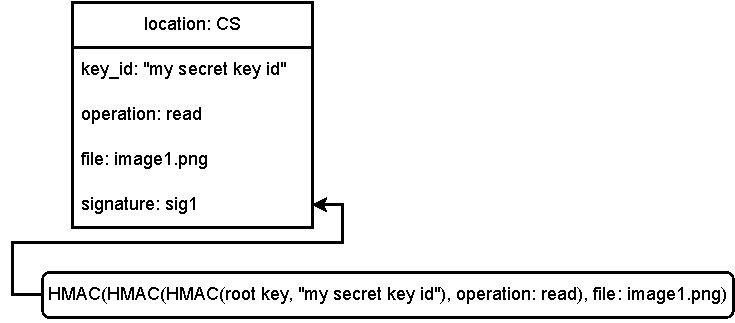
\includegraphics[width=0.8\textwidth]{images/basic_macaroon}}
    %popis obrazku
    \caption[Macaroons token]{Príklad jednoduchého Macaroons tokenu.}
    %id obrazku, pomocou ktoreho sa budeme na obrazok odvolavat
    \label{fig:macaroon_example}
\end{figure}

\subsection{Generovanie a delegácia Macaroons}

Každá cieľová služba disponuje tajným kľúčom, prípadne spôsobom ako ho vygenerovať. Ku každému tajnému kľúču musí vedieť odvodiť verejný nepriehľadný identifikátor, ktorý dokáže spätne previesť na tajný kľúč. Takého identifikátory môžu byť implementované napríklad ako náhodné príležitostné slová reprezentujúce kľúč v databáze alebo pomocou šifrovania s verejným alebo súkromným kľúčom \cite{macaroons_key_id}.

Cieľová služba vytvorí nový token z danej lokácie, identifikátora a tajného kľúča $sk$ tak, že podpíše identifikátor pomocou $sk$ a spojí lokáciu, identifikátor a podpis. Podpis vypočíta ako $HMAC(sk, identifikátor)$.

Takto vytvorený token si môžeme predstaviť ako zlatý kľúč, ktorý autorizuje ľubovoľnú požiadavku na cieľovú službu. Cieľová služba môže ďalej token poslať inej službe. Ako sme uviedli v úvode podkapitoly, každá služba môže token zoslabiť alebo kontextovo obmedziť pridaním pravidiel.

Pravidlá prvej strany pridá služba do tokenu $M$ tak, že pridá reťazec popisujúci pravidlo (tento reťazec označme $rule$) do tokenu a vypočíta nový podpis tokenu pomocou doterajšieho podpisu $M.signature$ ako $HMAC(M.signature, rule)$. Takto vytvoreným podpisom nahradí predchádzajúci podpis. Tento proces môže zopakovať viac krát a tým pridať ľubovoľný počet pravidiel.

Na pridanie pravidla tretej strany musí mať služba vzťah s danou službou tretej strany a dôverovať jej. Služba $A$ pridávajúca pravidlo vygeneruje koreňový kľúč pravidla $RK$ a potrebuje zabezpečiť, aby ho vedela zderivovať daná služba tretej strany $B$ ako aj cieľová služba $CS$. 

Prvý prípad môže služba $A$ zabezpečiť viacerými spôsobmi napríklad tak, že pošle kľúč a pravidlo službe $B$ cez zabezpečený kanál a tá jej vráti jeho identifikátor $cId$. Alebo ak zverejňuje služba $B$ verejný kľúč, prípadne služby zdieľajú tajný kľúč, môže služba $A$ vytvoriť $cId$ zašifrovaním $RK$ a pravidla pomocou šifrovacieho kľúča $cRK$ (verejný kľúč služby $B$ alebo zdieľaný tajný kľúč). Druhý prípad zabezpečí služba $A$ symetrickým zašifrovaním $RK$ pomocou podpisu tokenu. Takto vzniknutý reťazec označme $vId$.

Reťazec reprezentujúci pravidlo tretej stany je zreťazenie lokácie služby tretej strany, $cId$ a $vId$, označme tento reťazec $rule_B$. Služba $A$ vloží $rule_B$ do zoznamu pravidiel tokenu $M$ a vytvorí nový podpis tokenu pomocou aktuálneho podpisu tokenu $M.signature$ ako $HMAC(M.signature, rule_B)$. Príklad pridania pravidla tretej strany je na obrázku \ref{fig:add_caveat}. Služba tretej strany vie z $cId$ odvodiť koreňový kľúč pravidla, lebo $cId$ buď sama vytvorila alebo pozná kľúč na dešifrovanie $cId$. Cieľová služba pozná koreňový kľúč tokenu, teda si vie pomocou postupného podpisovania pravidiel odvodiť kľúč pre dešifrovanie $vId$ a dešifrovaním $vId$ získa koreňový kľúč pravidla.

\begin{figure}
    %vlozenie samotneho obrazku vycentrovaneho a vhodnej velkosti
    %obrazok je v subore images/session.png
    \centerline{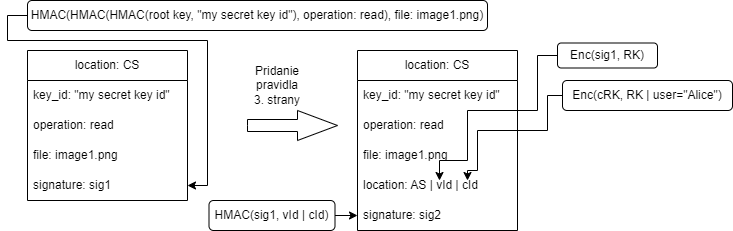
\includegraphics[width=0.8\textwidth]{images/3rd_party_caveat}}
    %popis obrazku
    \caption[Pridanie pravidla tretej strany]{Príklad pridania pravidla tretej strany, konkrétne pravidla \textit{user=``Alice''} na autentifikačný server (AS). $RK$ je koreňový kľúč pravidla a symbol | reprezentuje zreťazenie.}
    %id obrazku, pomocou ktoreho sa budeme na obrazok odvolavat
    \label{fig:add_caveat}
\end{figure}

Tvorba podpisu tokenu teda zodpovedá reťazovej aplikácií funkcie HMAC na identifikátor a pravidlá tokenu. Hešovanie je ireverzibilná operácia, preto nie je možné pravidlá odstraňovať, lebo nato by bolo potrebné vypočítať predchádzajúci podpis tokenu. To je možné iba podpísaním identifikátora koreňovým kľúčom a následným podpisovaním pravidiel vždy pomocou posledného podpisu ako kľúča.

\subsection{Vytvorenie požiadavky s Macaroons tokenom}
\label{sec:macaroon_request}

Služba komunikujúca s klientom pošle token klientovi. Na vytvorenie požiadavky autorizovanej týmto tokenom, musia byť splnené všetky pravidlá tokenu. Splnenie pravidiel prvej strany závisí od samotného kontextu požiadavky, no pre splnenie pravidiel tretej strany musí klient poskytnúť cieľovej službe dôkazy o ich splnení od daných služieb tretích strán.

Tieto dôkazy sú reprezentované \textit{vybíjacími tokenmi} (angl. discharge Macaroons). Vybíjacie tokeny majú rovnakú štruktúru aj postup generácie ako obyčajné Macaroons tokeny. Potom, čo klient obdrží Macaroons token, ho prehľadá pre všetky pravidlá tretích strán. Pre každé pravidlo tretej strany, pošle požiadavku na službu tretej strany s $cId$ daného pravidla. Služba tretej strany zderivuje koreňový kľúč pravidla a samotné pravidlo z $cId$. Následne môže vykonať akékoľvek opatrenia na overenie splnenia pravidla klientom, napríklad vyzvať klienta, aby zadal heslo. Ak je pravidlo splnené, vytvorí služba tretej strany vybíjací token z $cId$ pomocou koreňového kľúča pravidla. Následne môže pridať do vybíjacieho tokenu ľubovoľné ďalšie pravidlá vrátane pravidiel tretích strán. Potom podpis tokenu zahešuje (hešovaním bez kľúča), aby sa nedali do vybíjacieho tokenu pridávať ďalšie pravidlá. Nakoniec pošle vybíjací token klientovi. Príklad získania vybíjacieho tokenu je na obrázku \ref{fig:user_request}.

\begin{figure}
    %vlozenie samotneho obrazku vycentrovaneho a vhodnej velkosti
    %obrazok je v subore images/session.png
    \centerline{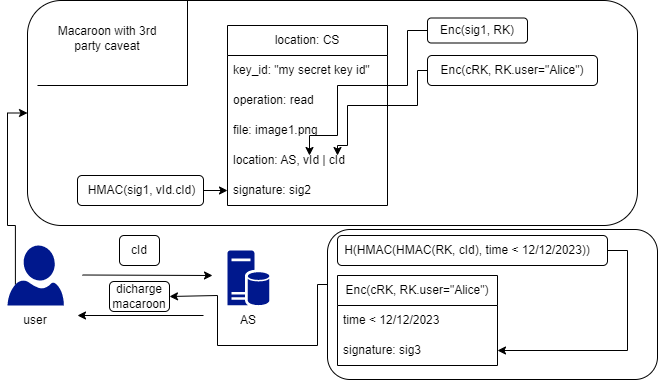
\includegraphics[width=0.8\textwidth]{images/user_request}}
    %popis obrazku
    \caption[Získanie vybíjacieho tokenu používateľom]{Príklad získania vybíjacieho tokenu používateľom. $RK$ je koreňový kľúč pravidla a symbol | reprezentuje zreťazenie.}
    %id obrazku, pomocou ktoreho sa budeme na obrazok odvolavat
    \label{fig:user_request}
\end{figure}

Keď klient získa vybíjací token pre každé pravidlo tretej strany, vytvorí požiadavku na cieľovú službu, ku ktorej priloží Macaroons token a všetky vybíjacie tokeny.

Vybíjacie tokeny sú silnými dôkazmi od tretích strán, dokazujú splnenie pravidla s rovnakým $cId$ a koreňovým kľúčom pravidla v každom Macaroons tokene. Ak by klient poslal požiadavku s vybíjacími tokenmi inej ako cieľovej službe (napríklad ako výsledok phishing útoku), táto služba môže jednoducho zneužiť vybíjacie tokeny klienta na dôkaz splnenia pravidiel vo vlastných tokenoch. Preto je potrebné aby klient vybíjacie tokeny zviazal s jeho Macaroons tokenom ešte predtým ako vytvorí požiadavku.

Zviazanie pôvodného Macaroons tokenu $M$ s vybíjacím tokenom $M'$ prebieha úpravou podpisu $M'$. Špecifikácia necháva otvorené, ako presne má táto úprava vyzerať. Jedna z možných implementácií by bola vytvoriť nový podpis $M'$ zahešovaním podpisov $M$ a $M'$ pomocou hešovacej funkcie bez kľúča (H), napríklad SHA-256. Nový podpis $M'.signature$ by sa potom vypočítal ako $M'.signature = H(M.signature, M'.signature)$.


\subsection{Spracovanie požiadavky cieľovou službou}

Predtým ako cieľová služba autorizuje požiadavku od klienta zvaliduje priložený Macaroons token. Pre úspešnú validáciu tokenu musia byť všetky pravidlá splnené a podpis tokenu korektný.

Splnenie pravidiel prvej strany overí cieľová služba overením splnenia predikátu každého pravidla v rámci kontextu požiadavky. Pravidlá tretej strany overí služba rekurzívne nasledovným postupom. Pre každé pravidlo nájde vybíjací token a z $vId$ pravidla zderivuje koreňový kľúč pravidla. Rekurzívne overí všetky pravidlá vo vybíjacom tokene a pomocou koreňového kľúča pravidla overí korektnosť podpisu vybíjacieho tokenu. Ak sú všetky pravidlá splnené a podpisy všetkých tokenov korektné, autorizuje služba požiadavku klienta.

\section{Biscuits}

Ako posledný predstavíme najmladší token rozoberaný v tejto práci. Biscuits token bol predstavený v roku 2021 v blogu od spoluautora z firmy Clever Cloud \cite{biscuits_blog}. Vo voľne dostupnom repozitári \cite{biscuits_git} nájdeme detailne popísanú motiváciu a vývoj tokenu. Pôvodne bol Biscuits implementovaný v jazyku Rust, no v súčasnosti je k dispozícii aj implementácia v ďalších jazykoch, všetky nájdeme v repozitári \cite{biscuits_git}.

Biscuits bol inšpirovaný Macaroons, implementuje podobnú schému zabezpečenia aj funkcionality. Rovnako dovoľuje delegovať autorizáciu medzi službami a ľubovoľná entita vlastniaca token ho môže \textit{zoslabiť} alebo aj \textit{kontextovo obmedziť}. Hlavným rozdielom oproti Macaroons je, že Biscuits tokeny používajú na postupné vytváranie podpisu asymetrické šifrovanie, konkrétne podpisovú funkciu Ed25519 \cite{ed_rfc}. Ďalším veľkým rozdielom je, že Biscuits používa na modelovanie práv, kontrol a dát v rámci tokenu špeciálny variant Datalogu bez negácie a na konkrétnych dátových typoch \cite{datalog_bis}.

Zoslabenie a kontextové obmedzenie tokenu sa realizuje pomocou pridania nového bloku. Blok môže pridať aj služba tretej strany, v takom prípadne budeme hovoriť o externom bloku.

\subsection{Štruktúra Biscuits}

Samotný token sa skladá z blokov a niektorých globálnych informácií pre celý token. Globálne informácie sú identifikátor koreňového verejného kľúča a dôkaz, ktorý slúži na pridávanie ďalšieho bloku. Každý token obsahuje autoritatívny blok, ktorý pridala služba vytvárajúca token.

Každý blok obsahuje serializovaný datalogový program, podpis bloku a verejný kľúč. V prípade, že ide o externý blok, aj podpis bloku službou tretej strany a príslušný verejný kľúč služby tretej strany. Príklad základného Biscuits tokenu je na obrázku \ref{fig:biscuits_token}.

Datalogový program sa skladá z faktov, pravidiel, kontrol a pomocných informácií, detailnú schému formátu nájdeme v súbore schema.proto repozitára \cite{biscuits_git}. Fakty a pravidlá sú bežné datalogové fakty a pravidlá. Kontroly sú množiny datalogových dotazov. Dotaz je splnený práve vtedy, keď je jeho výsledok aspoň jeden fakt. Kontrola je splnená práve vtedy, keď je splnený aspoň jeden dotaz z množiny dotazov danej kontroly. Okrem toho definuje Biscuits aj politiky, ktoré vytvára entita validujúca token. Viac sa politikám budeme venovať v nasledujúcej podkapitole. Bloky a politiky môžu mať anotáciu definujúcu, ktorým blokom dôverujú a teda s faktami a pravidlami, ktorých blokov pracujú. Vždy platí, že blok verí autoritatívnemu bloku, sebe a informáciám v službe validujúcej token. Anotáciou môže blok definovať, že dôveruje aj všetkým predchádzajúcim blokom alebo všetkým blokom podpísaným konkrétnym verejným kľúčom. Posledná možnosť sa využíva pre integráciu služieb tretích strán do autorizačnej schémy.
Datalogový program je serializovaný ako Protocol Buffer \cite{protobuf} podľa konkrétnej schémy definovanej v súbore schema.proto alebo v novšej verzii pomocou base64url kódovania \cite{base64_rfc}.

\begin{figure}
    %vlozenie samotneho obrazku vycentrovaneho a vhodnej velkosti
    %obrazok je v subore images/session.png
    \centerline{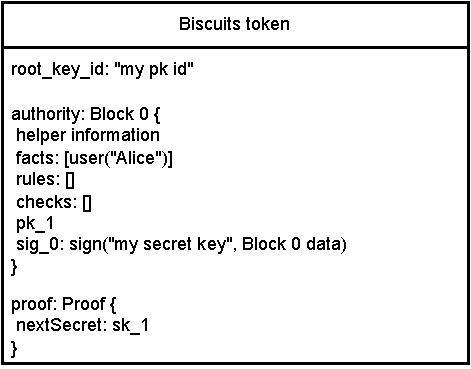
\includegraphics[width=0.5\textwidth]{images/biscuits_token2}}
    %popis obrazku
    \caption[Biscuits token]{Príklad Biscuits tokena s jediným blokom.}
    %id obrazku, pomocou ktoreho sa budeme na obrazok odvolavat
    \label{fig:biscuits_token}
\end{figure}

\subsection{Generovanie a delegácia autorizácie}

Na vygenerovanie nového Biscuits tokenu potrebuje služba dvojicu súkromného a verejného kľúča. Do tokenu vloží verejný kľúč alebo jeho identifikátor ako koreňový verejný kľúč daného tokenu. Vytvorí autoritatívny blok, do ktorého vloží základné fakty a pravidlá platné pre tento token. Následne vygeneruje novú dvojicu kľúčov $pk_1$ a $sk_1$. Kľúč $pk_1$ vloží do autoritatívneho bloku a $sk_1$ do dôkazu tokenu. Kľúč $sk_1$ bude slúžiť na podpísanie ďalšieho bloku tokenu a $pk_1$ na overenie tohto podpisu. Nakoniec celý autoritatívny blok podpíše súkromným koreňovým kľúčom a podpis vloží do bloku.

Takto vytvorený token môže služba poslať iným službám a tieto môžu pridávať ďalšie bloky a tým obmedzovať autorizačné práva tokenu. Na vytvorenie $i$-teho bloku potrebuje služba vygenerovať dvojicu kľúčov $pk_{i+1}$, $sk_{i+1}$, kde $pk_{i+1}$ vloží do bloku a $sk_{i+1}$ do dôkazu tokenu. Blok môže pridať aj služba tretej strany, v takom prípade musí vložiť aj podpis bloku služby tretej strany a verejný kľúč služby tretej strany. Celý blok následne podpíše kľúčom $sk_i$, ktorý vybrala z dôkazu tokenu pred jeho nahradením.

Ľubovoľná služba môže token zapečatiť a znemožniť tak pridávanie nových blokov. Zapečatenie tokenu pozostáva z podpísania posledného bloku kľúčom z dôkazu tokenu. Tento podpis sa vloží do dôkazu tokenu.

\subsection{Validácia Biscuits}

Služba validujúca Biscuits token musí vedieť odvodiť koreňový verejný kľúč tokenu z jeho identifikátora. Služba token deserializuje a postupne zvaliduje všetky podpisy tokenov. Podpis $i+1$-vého bloku validuje pomocou kľúča $pk_{i+1}$ vloženého vnútri $i$-teho bloku. Podpis autoritatívneho bloku validuje pomocou koreňového verejného kľúča a podpis služby tretej strany pomocou verejného kľúča danej služby uloženého vnútri daného bloku. Ak je token zapečatený validuje podpis v dôkaze tokenu pomocou verejného kľúča v poslednom bloku, ak token nie je zapečatený skontroluje, či verejný kľúč v poslednom bloku tvorí dvojicu so súkromným v dôkaze tokenu.

Ak je token validný, prebehnú postupne všetky kontroly v blokoch a to tak, že sa spustí daný datalogový program nad faktami a pravidlami podľa anotácie bloku a následne sa vykonajú dotazy v kontrolách. Fakty definuje aj samotná služba, napríklad vytvorí fakty na základe kontextu požiadavky. Príkladom takýchto faktov je typ operácie a IP adresa volajúceho. Token je validný iba ak sú splnené všetky kontroly. 

Okrem kontrol v rámci blokov tokenu môže validujúca služba definovať ďalšie kontroly a politiky a pravidlá. Pravidlá odvádzajú nové fakty len z faktov odvodených autoritatívnym blokom prípadne samotnou službou. Kontroly a politiky pracujú len nad faktami odvodenými autoritatívnym blokom a službou samotnou. Tieto kontroly musia byť tiež všetky splnené, aby bol token validný.

Politiky definujú väčšie kontroly, taktiež pozostávajú zo zoznamu dotazov. Delia sa na dva typy - povoľovacie a zamietacie politiky. Politika je splnená ak je splnený aspoň jeden dotaz danej politiky. Pri validácii tokenu sa vyhodnocujú politiky postupne po jednej. Ak je splnená povoľovacia politika, token je validný. Ak je splnená zamietacia politika alebo nie je splnená žiadna politika, token je nevalidný. Vyhodnocovanie končí s prvou splnenou politikou.

\subsection{Delegácia časti autorizácie na tretiu stranu}

Každá služba môže využiť inú službu na nejakú časť autorizácie. Na tento účel slúžia externé bloky. Ak chce služba $A$ delegovať autorizáciu na službu $B$, vytvorí blok s anotáciou obsahujúcou verejný kľúč služby $B$ a vytvorí kontrolu, ktorá používa fakty, ktoré vie zabezpečiť len služba $B$. Následne pošle službe $B$ informácie potrebné pre autorizáciu danej požiadavky službou $B$, ktorá vykoná ľubovoľné operácia nutné pre autorizáciu danej požiadavky a ak je úspešná vráti službe $A$ nový externý blok obsahujúci potrebné fakty a kontroly. 